%%%%%%%%%%%%%%%%%%%%%%%%%%%%%%%%%%%%%%%%%
% Jacobs Landscape Poster
% LaTeX Template
% Version 1.0 (29/03/13)
%
% Created by:
% Computational Physics and Biophysics Group, Jacobs University
% https://teamwork.jacobs-university.de:8443/confluence/display/CoPandBiG/LaTeX+Poster
% 
% Further modified by:
% Nathaniel Johnston (nathaniel@njohnston.ca)
%
% This template has been downloaded from:
% http://www.LaTeXTemplates.com
%
% License:
% CC BY-NC-SA 3.0 (http://creativecommons.org/licenses/by-nc-sa/3.0/)
%
%%%%%%%%%%%%%%%%%%%%%%%%%%%%%%%%%%%%%%%%%

%----------------------------------------------------------------------------------------
%	PACKAGES AND OTHER DOCUMENT CONFIGURATIONS
%----------------------------------------------------------------------------------------

\documentclass[final,table]{beamer}
\usepackage{xcolor}
\usepackage[scale=1.24]{beamerposter} % Use the beamerposter package for laying out the poster

\usetheme{confposter} % Use the confposter theme supplied with this template
\usepackage{graphicx}
\usepackage{caption}
\usepackage{subcaption}
\setbeamercolor{block title}{fg=ngreen,bg=white} % Colors of the block titles
\setbeamercolor{block body}{fg=black,bg=white} % Colors of the body of blocks
\setbeamercolor{block alerted title}{fg=white,bg=dblue!70} % Colors of the highlighted block titles
\setbeamercolor{block alerted body}{fg=black,bg=dblue!10} % Colors of the body of highlighted blocks
% Many more colors are available for use in beamerthemeconfposter.sty

%-----------------------------------------------------------
% Define the column widths and overall poster size
% To set effective sepwid, onecolwid and twocolwid values, first choose how many columns you want and how much separation you want between columns
% In this template, the separation width chosen is 0.024 of the paper width and a 4-column layout
% onecolwid should therefore be (1-(# of columns+1)*sepwid)/# of columns e.g. (1-(4+1)*0.024)/4 = 0.22
% Set twocolwid to be (2*onecolwid)+sepwid = 0.464
% Set threecolwid to be (3*onecolwid)+2*sepwid = 0.708

\newlength{\sepwid}
\newlength{\onecolwid}
\newlength{\twocolwid}
\newlength{\threecolwid}
\setlength{\paperwidth}{48in} % A0 width: 46.8in
\setlength{\paperheight}{36in} % A0 height: 33.1in
\setlength{\sepwid}{0.024\paperwidth} % Separation width (white space) between columns
\setlength{\onecolwid}{0.22\paperwidth} % Width of one column
\setlength{\twocolwid}{0.464\paperwidth} % Width of two columns
\setlength{\threecolwid}{0.708\paperwidth} % Width of three columns
\setlength{\topmargin}{-0.5in} % Reduce the top margin size
%-----------------------------------------------------------

\usepackage{graphicx}  % Required for including images

\usepackage{booktabs} % Top and bottom rules for tables
\definecolor{color1}{HTML}{FF66CC}
\definecolor{color2}{HTML}{4D90FE}
\definecolor{green}{HTML}{99FF99}
\definecolor{red}{HTML}{FF9999}
\definecolor{yellow}{HTML}{FFFF99}
\newcommand{\spar}{\vspace{26pt}\noindent}

%----------------------------------------------------------------------------------------
%	TITLE SECTION 
%----------------------------------------------------------------------------------------

\title{ Box Office Success Prediction based on Movie Attributes \hspace{1ex} 
          
\includegraphics[width=8ex]{logo.png}}
          
\author{Jonathan Sumrall and Natalia Kuznetsova } % Author(s)

\institute{Technical University of Eindhoven} % Institution(s)

%----------------------------------------------------------------------------------------

\begin{document}

\addtobeamertemplate{block end}{}{\vspace*{2ex}} % White space under blocks
\addtobeamertemplate{block alerted end}{}{\vspace*{2ex}} % White space under highlighted (alert) blocks

\setlength{\belowcaptionskip}{2ex} % White space under figures
\setlength\belowdisplayshortskip{2ex} % White space under equations

\begin{frame}[t] % The whole poster is enclosed in one beamer frame

\begin{columns}[t] % The whole poster consists of three major columns, the second of which is split into two columns twice - the [t] option aligns each column's content to the top




\begin{column}{\twocolwid} % The first column

\begin{block}{Goal}
\centering
\emph{Using only the attributes of a movie, predict whether or not it will be a success in the box office. }
\newline
\end{block}

\begin{block}{Data}
We collected data from IMDB.com, who provide their database in a human-readable list (LST) format. IMDBPy builds a SQL database from the data, and provides methods for querying the data.  We make a new collection of only the movies which contain the attributes we are interested in. 

\begin{figure}
          \includegraphics[width=70ex]{datafigure.pdf}
          \caption{Data collection process}
\end{figure}

We give a score to each movie in our collection based on how many famous actors were in the movie, how experienced the director is, and whether or not the movie premiers near a holiday. 

\begin{figure}
          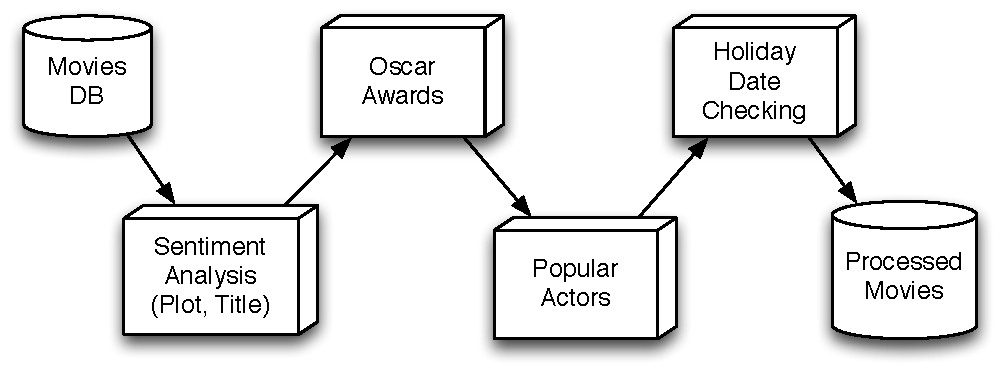
\includegraphics[width=50ex]{dataProcessingFigure.pdf}
          \caption{Scoring movies based on actors, director experience, and premier date.}
\end{figure}
\end{block}

\begin{block}{Sentiment analysis}
The plots on the IMDB web site are written by users, therefore we hypothesize that they contain emotional sentiment. We apply Sentiment Analysis on the plots to convert them to a numerical representation. Two approaches were tried and compared. \\

	\begin{table}
	    \begin{tabular}{|p{0.5\textwidth}|p{0.5\textwidth}|}
	    \hline
	   	\textbf{NLTK Approach} & \textbf{Web search approach} \\ \hline
	    Use Natural Language Toolkit's Naive Bayes Classifier & Compute average  semantic orientation with the use of web search engine queries \\ \hline
	    \cellcolor{yellow} 2000 training set from NLTK corpus & \cellcolor{green} the Internet as a training set \\ \hline
	    Query words after tokenization & Query phrases\\ \hline
	    Take the proportion of positive and negative  frequencies & Take the distance from positive and negative evaluation\\ \hline
	    \cellcolor{yellow} The size of training set & \cellcolor{red} The number of queries is restricted\\ \hline
	    \end{tabular} 
	    \end{table} 
    
\spar Due to the restriction the NLTK approach was chosen. Although the movie plot descriptions are written by users, the sentiment analysis does not make sense since the estimates are around 0  and hence there is no correlation between the plot and movie success. 
    
\end{block}
\end{column}
\begin{column}{\twocolwid} % The second column

\begin{block}{Classification}

From our collection of movies, we try to classify them as either a Success or a Failure. An accurate definition of a movie's box office success is difficult to make, as a successful movie could have a long and profitable run in theaters after the first weekend, it could have excellent DVD sales, or it could be syndicated on television for years later. It could have all of these but not have a very profitable opening weekend. 
We label success as: \emph{Opening Weekend Gross} $  > Budget* 0.3 $
The best classification algorithms for this problem are Gradient Boosting and K Nearest Neighbors. 
The Python library Scikit-Learn was used for the implementation of the machine learning algorithms. 
The probability of correctly classifying a movie is 64\% with Gradient Boosting and 60\% with K Nearest Neighbors. 

\begin{figure}
\begin{subfigure}[b]{0.2\textwidth}
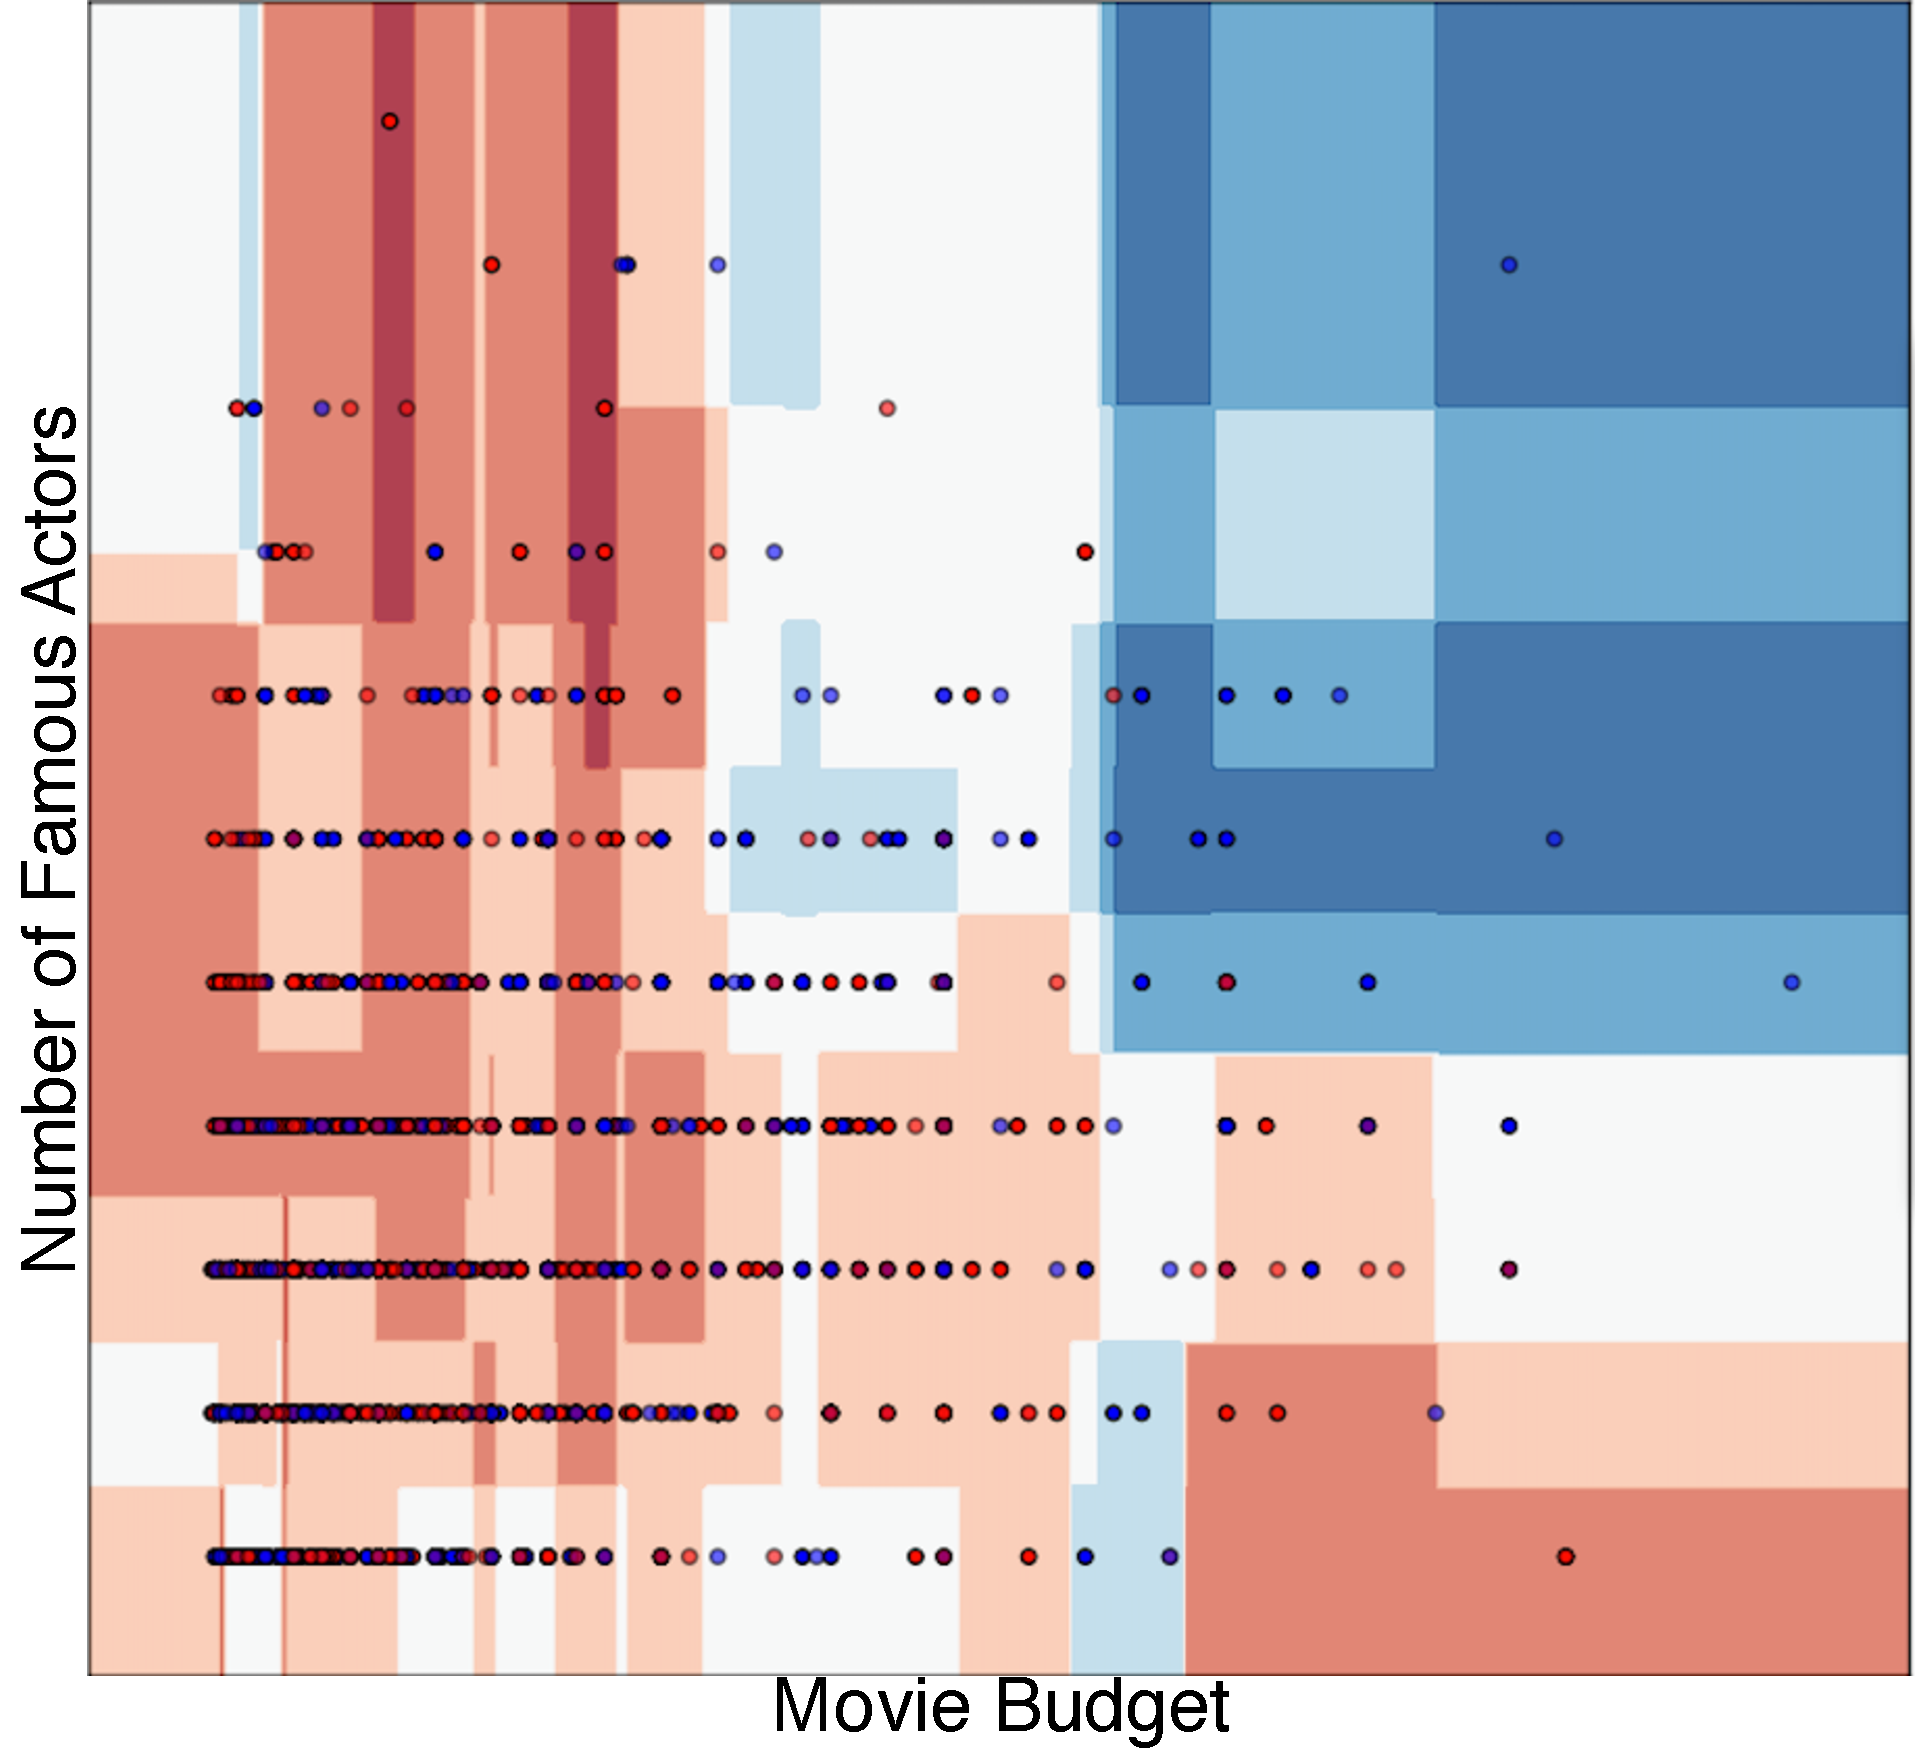
\includegraphics[width=30ex]{gb2.pdf}
\caption{Gradient Boosting}
\end{subfigure} \hspace{20ex}
\begin{subfigure}[b]{0.2\textwidth}
 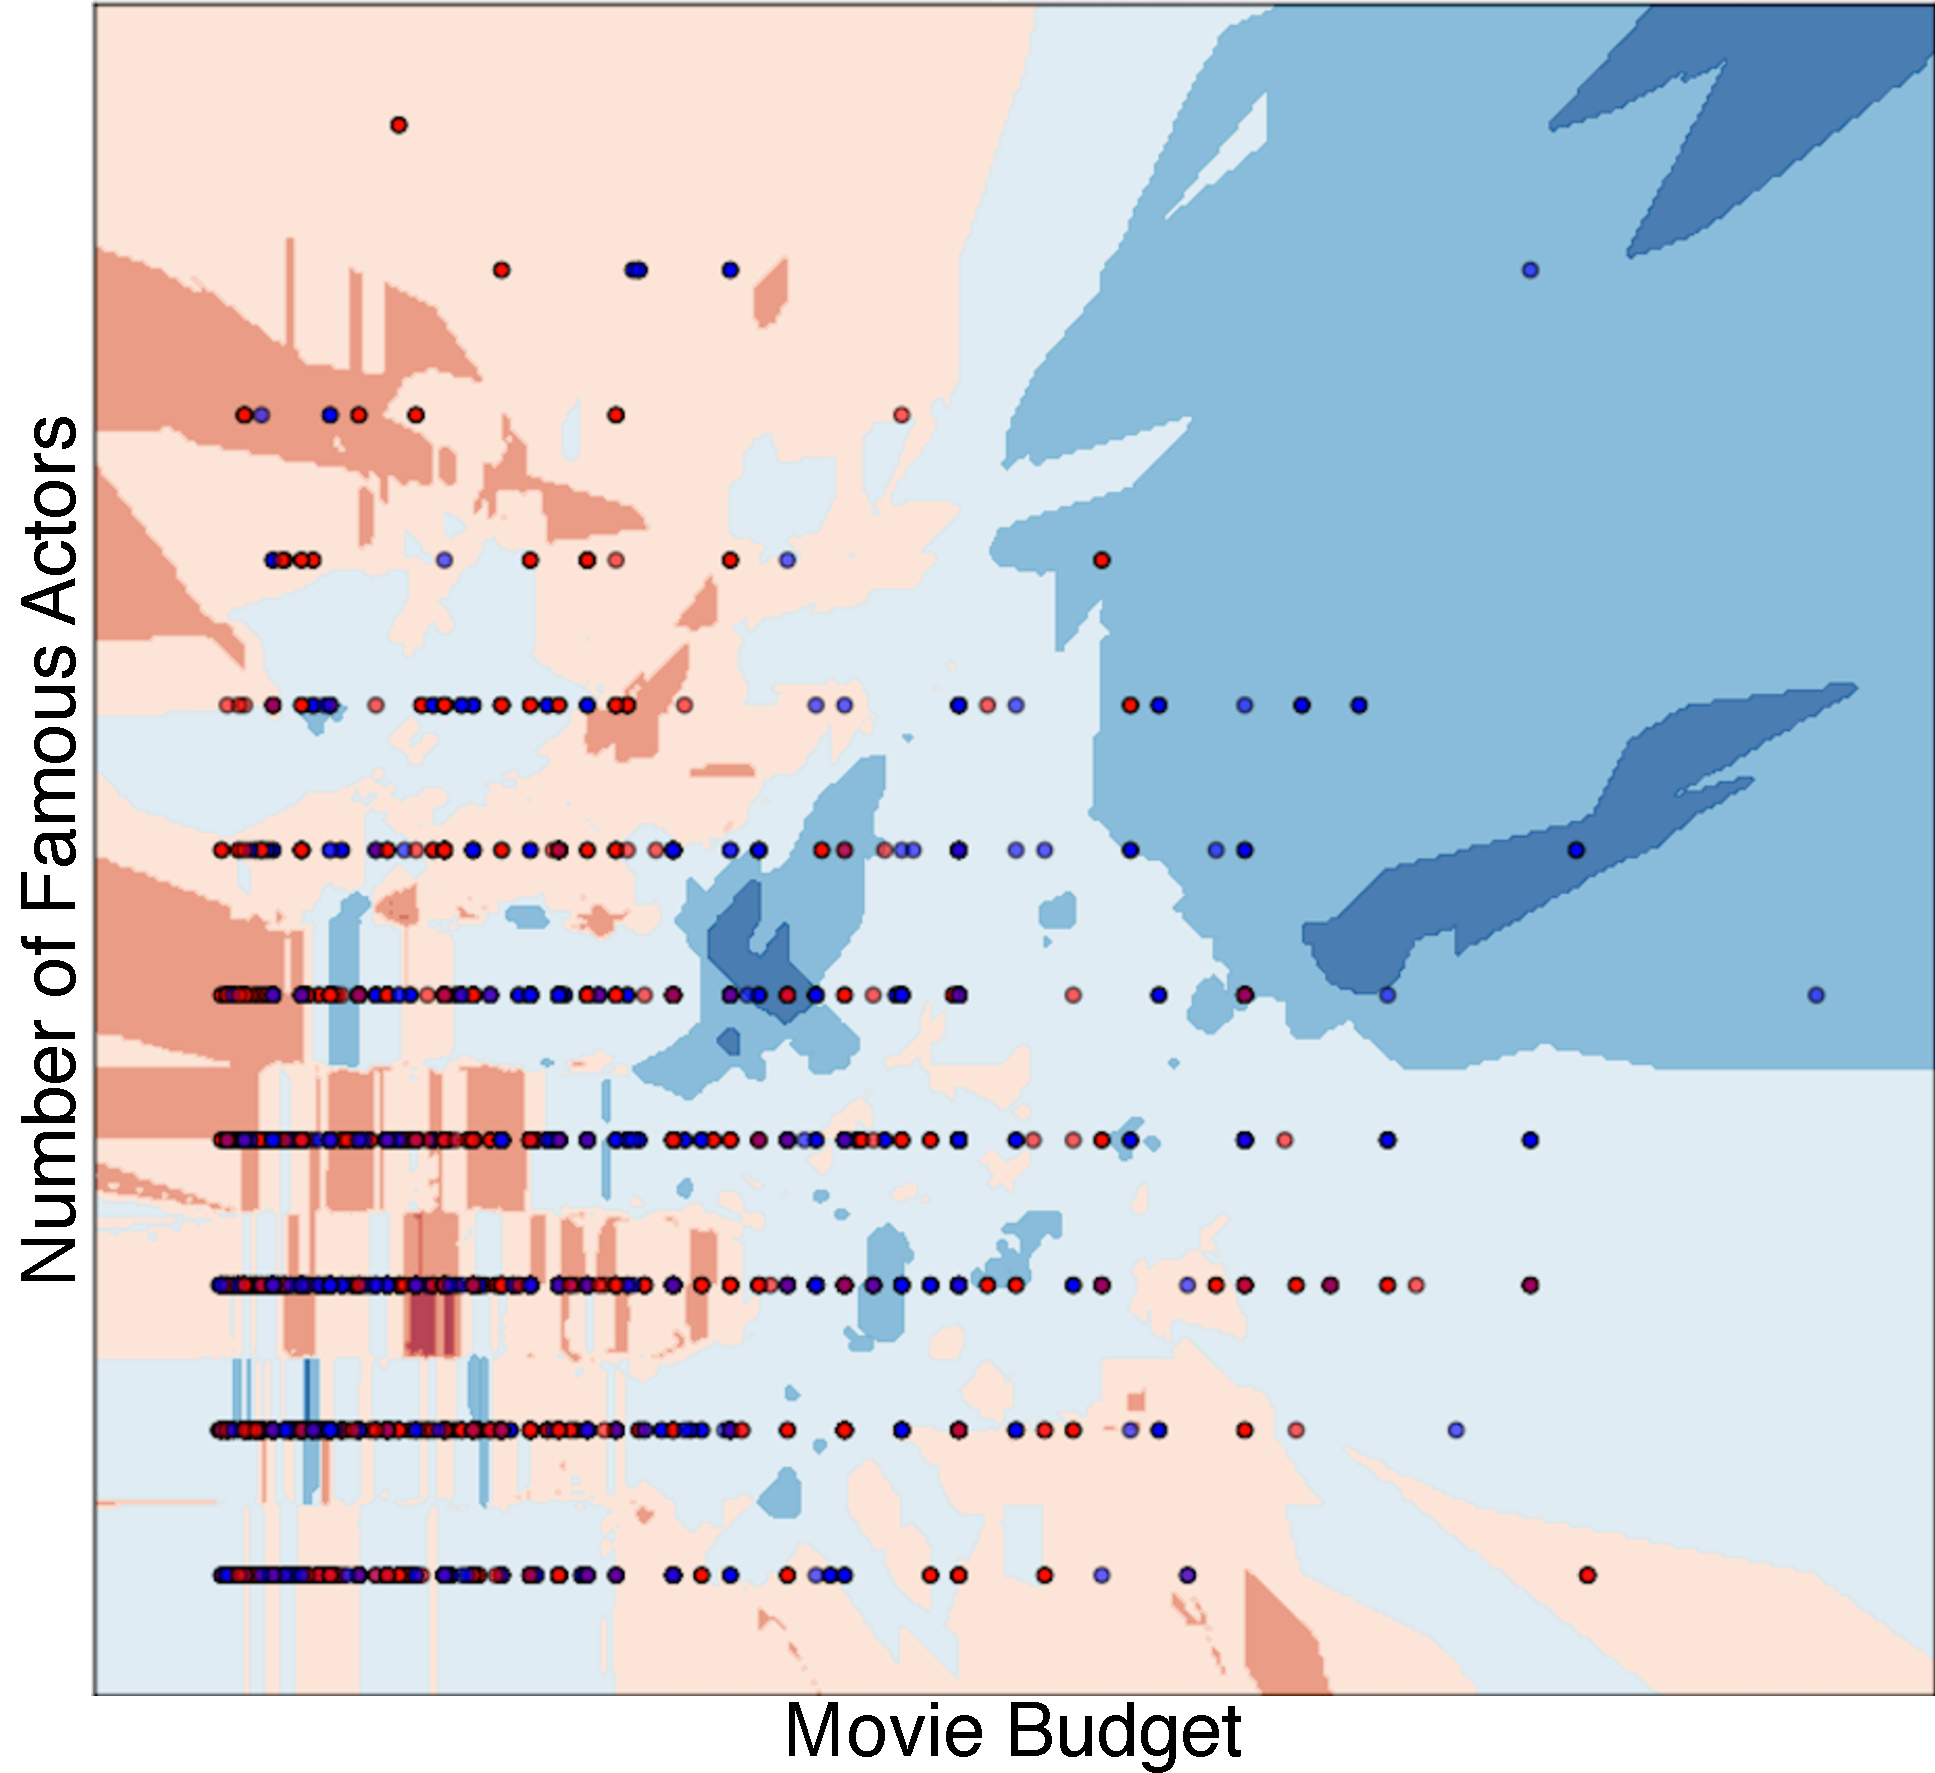
\includegraphics[width=30ex]{kn2.pdf}
 \caption{KNeighbors, K=15}
 \end{subfigure}
 \caption{Classification of movies, Blue is success}
\end{figure} 
\end{block}
\begin{block}{Tool and Features}
The tool is a web site where users can enter information about a movie including a title, budget, premier date, director, cast, and a plot description. It is necessary to enter the names correctly, thus the functions of autocorrection and autocompletion is essential.  

\begin{figure}\hspace{-10ex}
	\begin{subfigure}[b]{0.2\textwidth}
          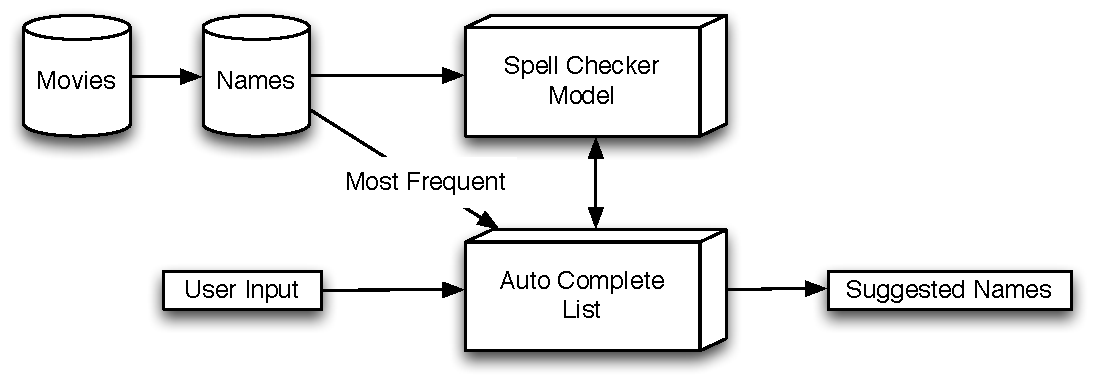
\includegraphics[width=40ex]{nameFig.pdf}
          \caption{Autocomplete and autocorrect procedure}
          \end{subfigure}\hspace{30ex}
          \begin{subfigure}[b]{0.2\textwidth}
          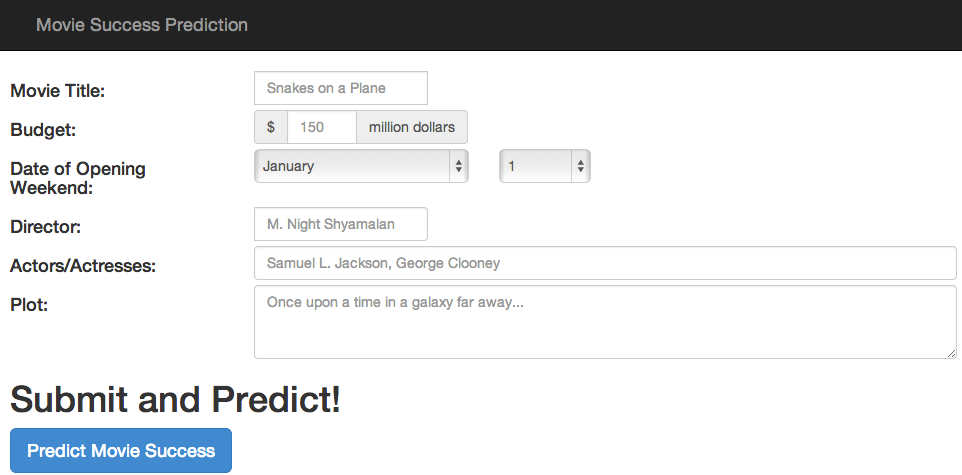
\includegraphics[width=40ex]{toolSS.png}
          \end{subfigure}
\end{figure}

\end{block}

\begin{block}{Conclusions}
\emph{The tool predicts the success of the described movie with an accuracy greater than random or na\"{\i}ve guessing. But overall the prediction is not as accurate as we thought it would be. There are other aspects of the data which could analyzed to yield better results, and a movie's success depends on other factors not included in the movie's attributes.}
\end{block}


\end{column}
\end{columns} % End of all the columns in the poster
\end{frame} % End of the enclosing frame
\end{document}